\begin{frame}{$d(K^-, n \pi^{\mp})"\Sigma^{\pm}"$ フィッティング  $\d(K^-, n)"X" : 1.44\sim1.52 [GeV/c^2]$}
  \label{page:fitKNpi2}
  
  \tminipageFour{
    \begin{figure}
      \centering
      \tiny
      $d(K^-, n)"X" : 1.44 \sim 1.45 [GeV/c^{2}]$
      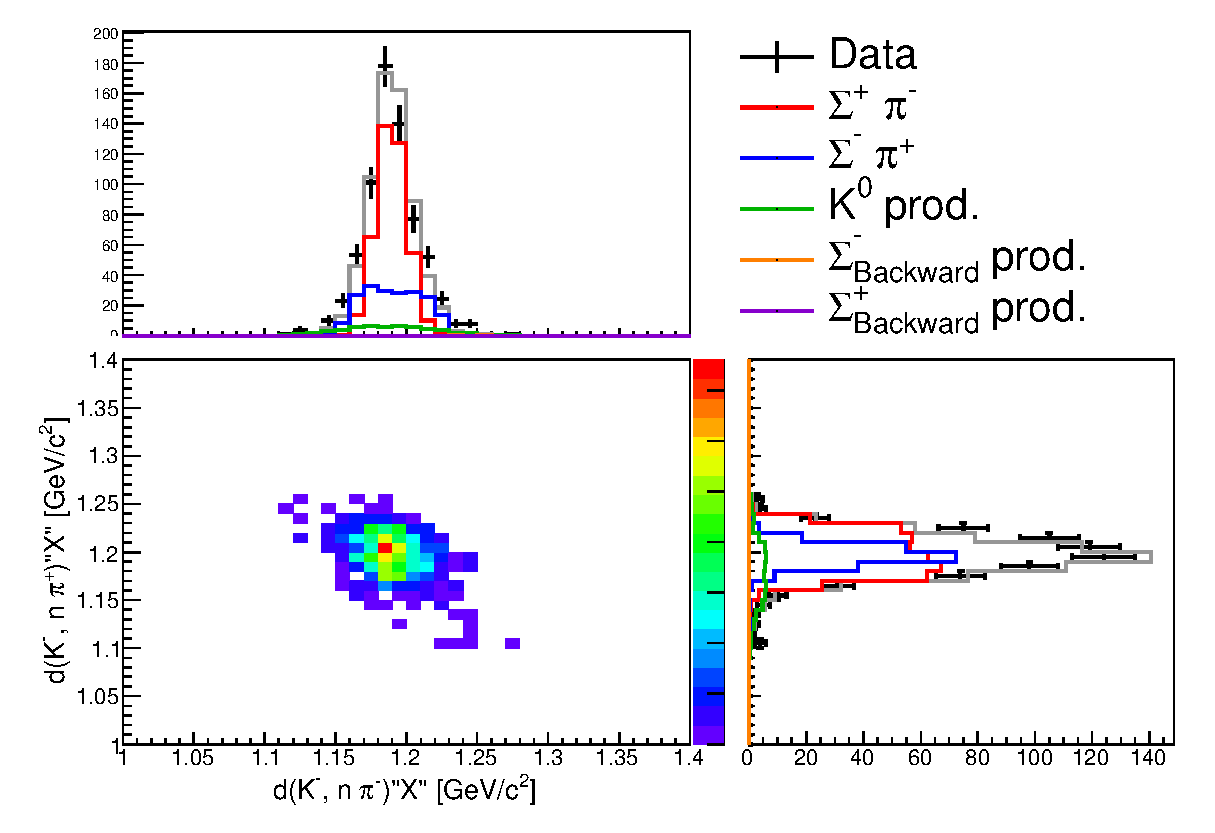
\includegraphics[width=2.5cm]{../pic/Run78/KN_ana_NC170_2sigma/KNpi_MM_9.eps}
    \end{figure}
  }{
    \begin{figure}
      \centering
      \tiny
      $d(K^-, n)"X" : 1.45 \sim 1.46 [GeV/c^{2}]$
      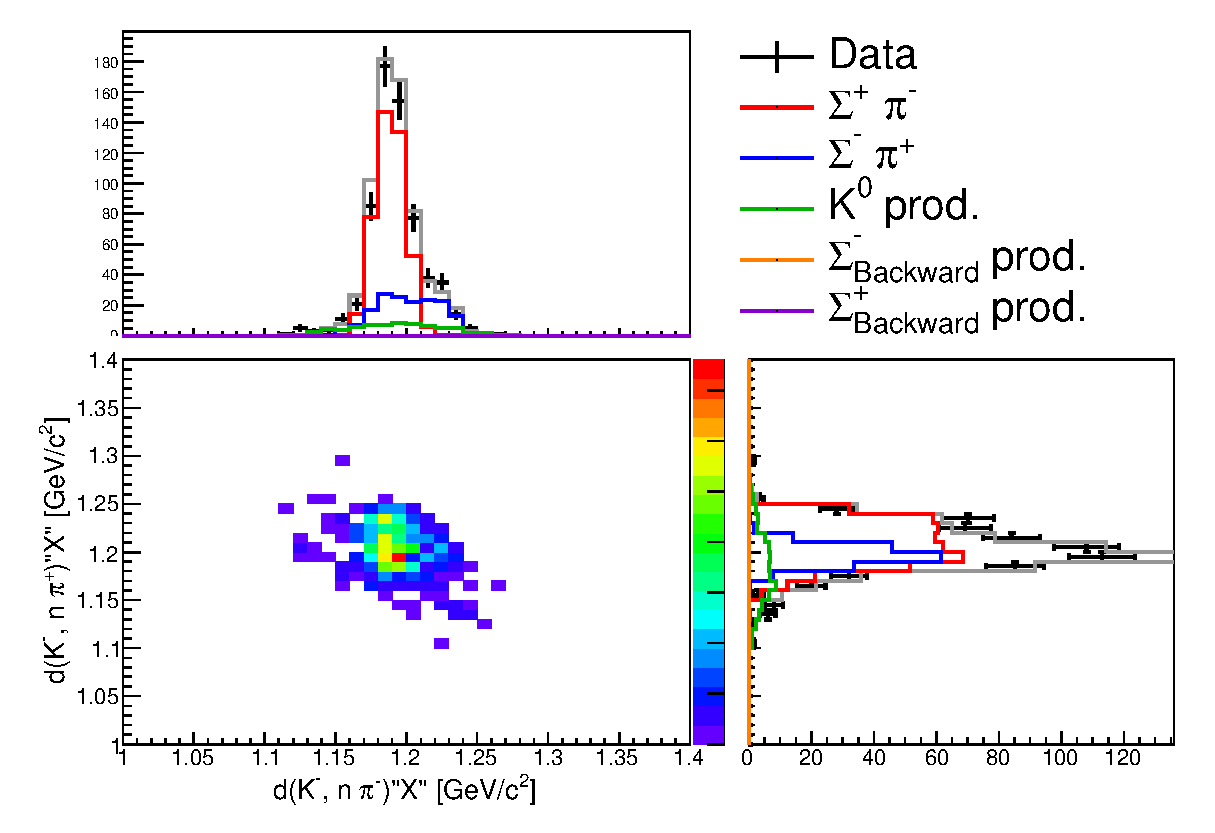
\includegraphics[width=2.5cm]{../pic/Run78/KN_ana_NC170_2sigma/KNpi_MM_10.eps}
    \end{figure}
  }{
    \begin{figure}
      \centering
      \tiny
      $d(K^-, n)"X" : 1.46 \sim 1.47 [GeV/c^{2}]$
      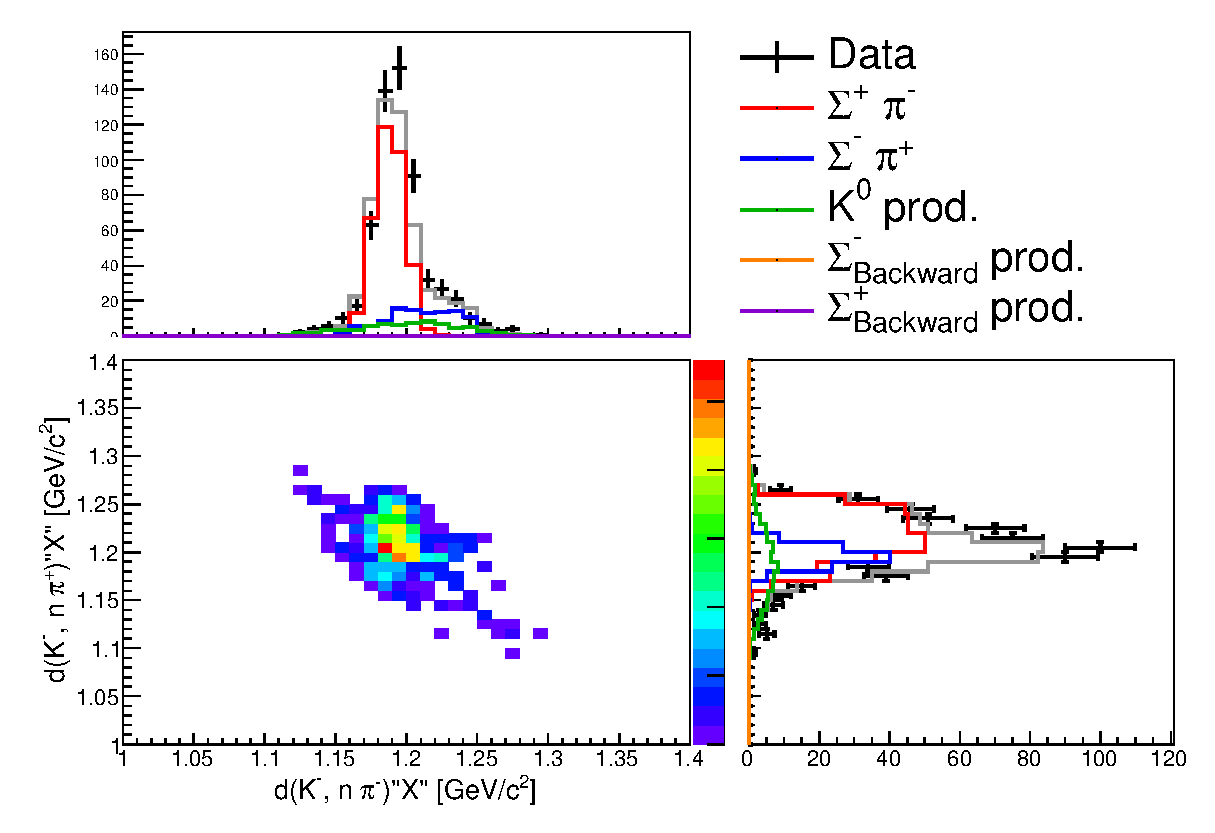
\includegraphics[width=2.5cm]{../pic/Run78/KN_ana_NC170_2sigma/KNpi_MM_11.eps}
    \end{figure}
  }{
    \begin{figure}
      \centering
      \tiny
      $d(K^-, n)"X" : 1.47 \sim 1.48 [GeV/c^{2}]$
      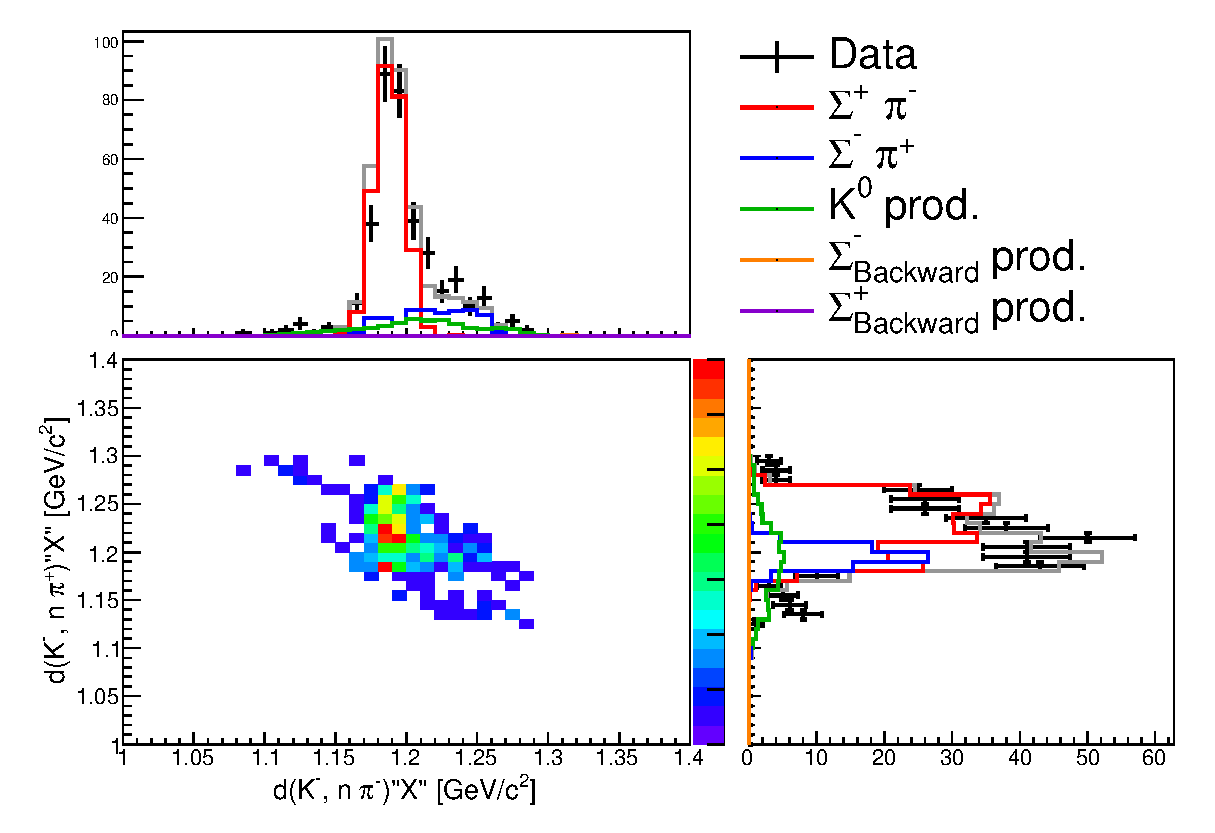
\includegraphics[width=2.5cm]{../pic/Run78/KN_ana_NC170_2sigma/KNpi_MM_12.eps}
    \end{figure}
  }

  \tminipageFour{
    \begin{figure}
      \centering
      \tiny
      $d(K^-, n)"X" : 1.48 \sim 1.49 [GeV/c^{2}]$
      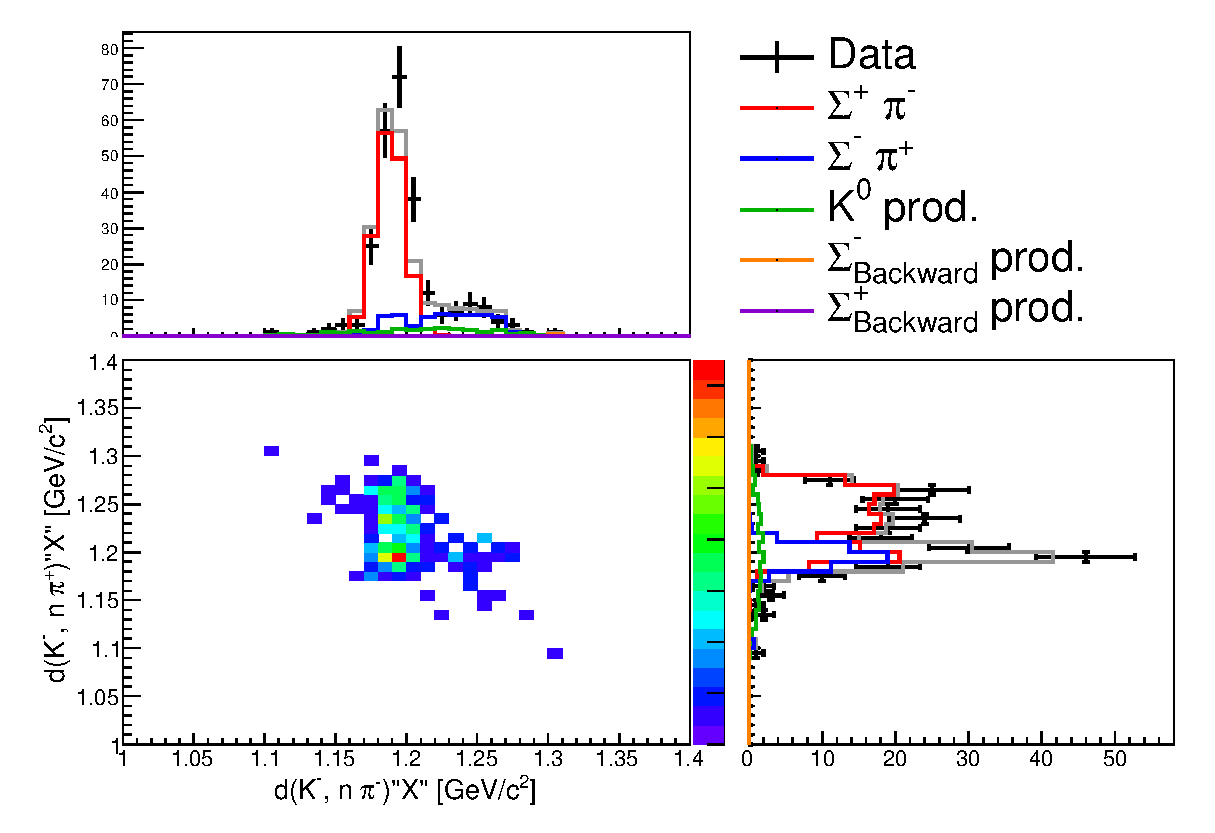
\includegraphics[width=2.5cm]{../pic/Run78/KN_ana_NC170_2sigma/KNpi_MM_13.eps}
    \end{figure}

  }{
    \begin{figure}
      \centering
      \tiny
      $d(K^-, n)"X" : 1.49 \sim 1.50 [GeV/c^{2}]$
      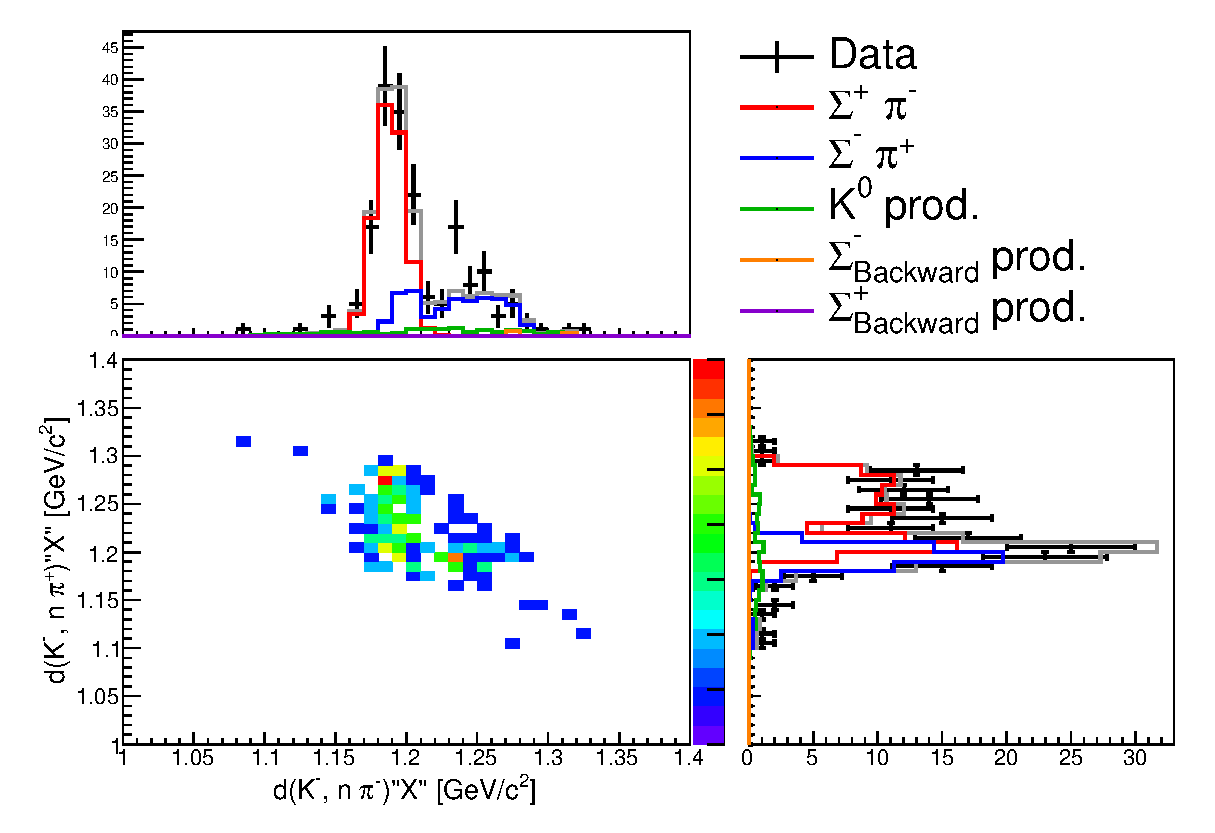
\includegraphics[width=2.5cm]{../pic/Run78/KN_ana_NC170_2sigma/KNpi_MM_14.eps}
    \end{figure}
  }{
    \begin{figure}
      \centering
      \tiny
      $d(K^-, n)"X" : 1.50 \sim 1.51 [GeV/c^{2}]$
      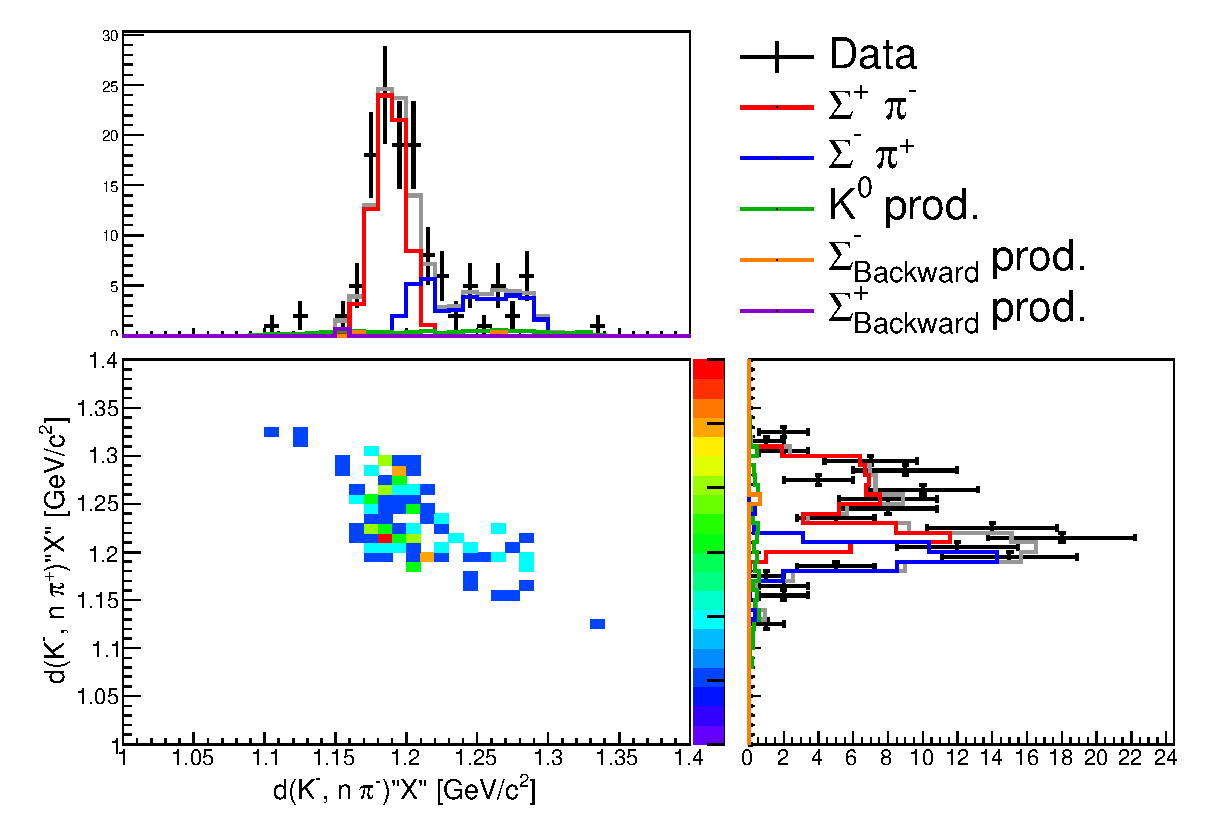
\includegraphics[width=2.5cm]{../pic/Run78/KN_ana_NC170_2sigma/KNpi_MM_15.eps}
    \end{figure}
  }{
    \begin{figure}
      \centering
      \tiny
      $d(K^-, n)"X" : 1.51 \sim 1.52 [GeV/c^{2}]$
      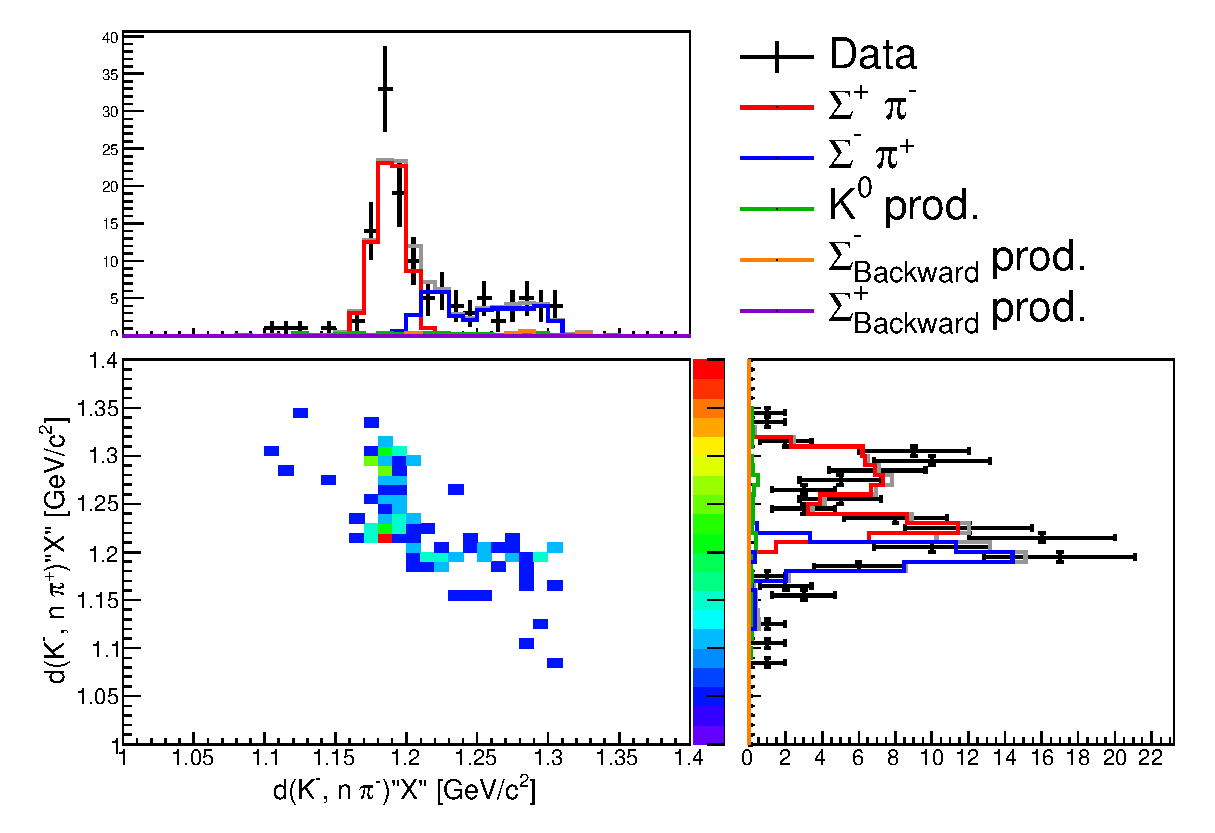
\includegraphics[width=2.5cm]{../pic/Run78/KN_ana_NC170_2sigma/KNpi_MM_16.eps}
    \end{figure}
  }
\end{frame}
